\documentclass[9pt,ignorenonframetext,]{beamer}

\setbeamertemplate{caption}[numbered]
\setbeamertemplate{caption label separator}{: }
\setbeamercolor{caption name}{fg=normal text.fg}
\beamertemplatenavigationsymbolsempty
\usepackage{lmodern}
\usepackage{amssymb,amsmath}
\usepackage{ifxetex,ifluatex}
\usepackage{fixltx2e} % provides \textsubscript
\ifnum 0\ifxetex 1\fi\ifluatex 1\fi=0 % if pdftex
  \usepackage[T1]{fontenc}
  \usepackage[utf8]{inputenc}
\else % if luatex or xelatex
  \ifxetex
    \usepackage{mathspec}
  \else
    \usepackage{fontspec}
  \fi
  \defaultfontfeatures{Ligatures=TeX,Scale=MatchLowercase}
\fi
% use upquote if available, for straight quotes in verbatim environments
\IfFileExists{upquote.sty}{\usepackage{upquote}}{}
% use microtype if available
\IfFileExists{microtype.sty}{%
\usepackage{microtype}
\UseMicrotypeSet[protrusion]{basicmath} % disable protrusion for tt fonts
}{}
\newif\ifbibliography
\hypersetup{
            pdftitle={Project 2: Augmenting functional information about human genes using probabilistic phylogenetic modeling},
            pdfauthor={George G. Vega Yon vegayon@usc.edu},
            pdfborder={0 0 0},
            breaklinks=true}
\urlstyle{same}  % don't use monospace font for urls
\usepackage{color}
\usepackage{fancyvrb}
\newcommand{\VerbBar}{|}
\newcommand{\VERB}{\Verb[commandchars=\\\{\}]}
\DefineVerbatimEnvironment{Highlighting}{Verbatim}{commandchars=\\\{\}}
% Add ',fontsize=\small' for more characters per line
\usepackage{framed}
\definecolor{shadecolor}{RGB}{48,48,48}
\newenvironment{Shaded}{\begin{snugshade}}{\end{snugshade}}
\newcommand{\KeywordTok}[1]{\textcolor[rgb]{0.94,0.87,0.69}{#1}}
\newcommand{\DataTypeTok}[1]{\textcolor[rgb]{0.87,0.87,0.75}{#1}}
\newcommand{\DecValTok}[1]{\textcolor[rgb]{0.86,0.86,0.80}{#1}}
\newcommand{\BaseNTok}[1]{\textcolor[rgb]{0.86,0.64,0.64}{#1}}
\newcommand{\FloatTok}[1]{\textcolor[rgb]{0.75,0.75,0.82}{#1}}
\newcommand{\ConstantTok}[1]{\textcolor[rgb]{0.86,0.64,0.64}{\textbf{#1}}}
\newcommand{\CharTok}[1]{\textcolor[rgb]{0.86,0.64,0.64}{#1}}
\newcommand{\SpecialCharTok}[1]{\textcolor[rgb]{0.86,0.64,0.64}{#1}}
\newcommand{\StringTok}[1]{\textcolor[rgb]{0.80,0.58,0.58}{#1}}
\newcommand{\VerbatimStringTok}[1]{\textcolor[rgb]{0.80,0.58,0.58}{#1}}
\newcommand{\SpecialStringTok}[1]{\textcolor[rgb]{0.80,0.58,0.58}{#1}}
\newcommand{\ImportTok}[1]{\textcolor[rgb]{0.80,0.80,0.80}{#1}}
\newcommand{\CommentTok}[1]{\textcolor[rgb]{0.50,0.62,0.50}{#1}}
\newcommand{\DocumentationTok}[1]{\textcolor[rgb]{0.50,0.62,0.50}{#1}}
\newcommand{\AnnotationTok}[1]{\textcolor[rgb]{0.50,0.62,0.50}{\textbf{#1}}}
\newcommand{\CommentVarTok}[1]{\textcolor[rgb]{0.50,0.62,0.50}{\textbf{#1}}}
\newcommand{\OtherTok}[1]{\textcolor[rgb]{0.94,0.94,0.56}{#1}}
\newcommand{\FunctionTok}[1]{\textcolor[rgb]{0.94,0.94,0.56}{#1}}
\newcommand{\VariableTok}[1]{\textcolor[rgb]{0.80,0.80,0.80}{#1}}
\newcommand{\ControlFlowTok}[1]{\textcolor[rgb]{0.94,0.87,0.69}{#1}}
\newcommand{\OperatorTok}[1]{\textcolor[rgb]{0.94,0.94,0.82}{#1}}
\newcommand{\BuiltInTok}[1]{\textcolor[rgb]{0.80,0.80,0.80}{#1}}
\newcommand{\ExtensionTok}[1]{\textcolor[rgb]{0.80,0.80,0.80}{#1}}
\newcommand{\PreprocessorTok}[1]{\textcolor[rgb]{1.00,0.81,0.69}{\textbf{#1}}}
\newcommand{\AttributeTok}[1]{\textcolor[rgb]{0.80,0.80,0.80}{#1}}
\newcommand{\RegionMarkerTok}[1]{\textcolor[rgb]{0.80,0.80,0.80}{#1}}
\newcommand{\InformationTok}[1]{\textcolor[rgb]{0.50,0.62,0.50}{\textbf{#1}}}
\newcommand{\WarningTok}[1]{\textcolor[rgb]{0.50,0.62,0.50}{\textbf{#1}}}
\newcommand{\AlertTok}[1]{\textcolor[rgb]{1.00,0.81,0.69}{#1}}
\newcommand{\ErrorTok}[1]{\textcolor[rgb]{0.76,0.75,0.62}{#1}}
\newcommand{\NormalTok}[1]{\textcolor[rgb]{0.80,0.80,0.80}{#1}}
\usepackage{longtable,booktabs}
\usepackage{caption}
% These lines are needed to make table captions work with longtable:
\makeatletter
\def\fnum@table{\tablename~\thetable}
\makeatother

% Prevent slide breaks in the middle of a paragraph:
\widowpenalties 1 10000
\raggedbottom


\setlength{\parindent}{0pt}
\setlength{\parskip}{6pt plus 2pt minus 1pt}
\setlength{\emergencystretch}{3em}  % prevent overfull lines
\providecommand{\tightlist}{%
  \setlength{\itemsep}{0pt}\setlength{\parskip}{0pt}}
\setcounter{secnumdepth}{0}
\usebackgroundtemplate{\includegraphics[width=\paperwidth,height=\paperheight]{/usr/local/lib/R/site-library/uscimage/templates/uscimage_pptx_background.jpg}}

\usepackage{tikz}

\newcommand{\includetikz}[2]{
\begin{figure}
\scalebox{#2}{
\input{#1}
}
\end{figure}
}

% Mathematical functions
\newcommand{\isone}[1]{{\boldsymbol{1}\left( #1 \right)}}
\renewcommand{\Pr}[1]{{\mbox{Pr}\left(#1\right) }}
\newcommand{\f}[1]{{f\left(#1\right) }}
\newcommand{\Prcond}[2]{{\mbox{Pr}\left(#1\vphantom{#2}\;\right|\left.\vphantom{#1}#2\right)}}
\newcommand{\fcond}[2]{{f\left(#1|#2\right) }}
\newcommand{\Expected}[1]{{\mathbb{E}\left\{#1\right\}}}
\newcommand{\likelihood}[2]{\mbox{L}\left(#1\vphantom{#2}\right|\left.\vphantom{#1}#2\right)}

% Mathematical Annotation -------------------------------
% Modify this so that it matches the P01 convention overall

% Tree
\newcommand{\phylo}{\Lambda{}} % The actual tree
\newcommand{\aphylo}{D{}}      % The annotated phylogenetic tree
\newcommand{\aphyloObs}{\tilde \aphylo{}} % The observed annotated phylogenetic tree

% Annotations
\newcommand{\Ann}{Z{}} % Matrix of "real" annotations
\newcommand{\ann}{z{}} % single element of "real" annotations

% Obs Annotations
\newcommand{\AnnObs}{X{}}
\newcommand{\annObs}{x{}}

% Pred. Annotations
\newcommand{\AnnPred}{\hat Z{}}
\newcommand{\annPred}{\hat z{}}

% Leaf nodes
\newcommand{\Leaf}{L{}}

% Shortest path
\newcommand{\Geodesic}{\mbox{T}{}}
\newcommand{\geodesic}{\tau{}}


% tricks for two column
\def\begincols{\begin{columns}[T]}
\def\begincol{\begin{column}[T]}
\def\endcol{\end{column}}
\def\endcols{\end{columns}}
% Copyright 2007 by Till Tantau
% Copyright 2012,2015 by Vedran Mileti\'c, Joseph Wright
%
% This file may be distributed and/or modified
%
% 1. under the LaTeX Project Public License and/or
% 2. under the GNU Public License.
%
% See the file doc/licenses/LICENSE for more details.

\mode<presentation>

% \definecolor{beamer@blendedblue}{rgb}{0.2,0.2,0.7} % use structure theme to change
\definecolor{USCCardinal}{HTML}{990000}
\definecolor{USCGold}{HTML}{FFCC00}
\definecolor{USCGray}{HTML}{CCCCCC}

\setbeamercolor{normal text}{fg=black,bg=white}
\setbeamercolor{alerted text}{fg=USCCardinal}
\setbeamercolor{example text}{fg=green!50!black}

% \setbeamercolor{structure}{fg=beamer@blendedblue}
\setbeamercolor{structure}{fg=USCCardinal}

\setbeamercolor{background canvas}{parent=normal text}
\setbeamercolor{background}{parent=background canvas}

\setbeamercolor{palette primary}{use=structure,fg=structure.fg}
\setbeamercolor{palette secondary}{use=structure,fg=structure.fg!75!black}
\setbeamercolor{palette tertiary}{use=structure,fg=structure.fg!50!black}
\setbeamercolor{palette quaternary}{fg=black}

\setbeamercolor{palette sidebar primary}{use=normal text,fg=normal text.fg}
\setbeamercolor{palette sidebar secondary}{use=structure,fg=structure.fg}
\setbeamercolor{palette sidebar tertiary}{use=normal text,fg=normal text.fg}
\setbeamercolor{palette sidebar quaternary}{use=structure,fg=structure.fg}

\setbeamercolor{math text}{}
\setbeamercolor{math text inlined}{parent=math text}
\setbeamercolor{math text displayed}{parent=math text}

\setbeamercolor{normal text in math text}{}

\setbeamercolor{local structure}{parent=structure}

\setbeamercolor{titlelike}{parent=structure}

\setbeamercolor{title}{parent=titlelike}
\setbeamercolor{title in head/foot}{parent=palette quaternary}
\setbeamercolor{title in sidebar}{parent=palette sidebar quaternary}

\setbeamercolor{subtitle}{parent=title}

\setbeamercolor{author}{}
\setbeamercolor{author in head/foot}{parent=palette primary}
\setbeamercolor{author in sidebar}{use=palette sidebar tertiary,fg=palette sidebar tertiary.fg}

\setbeamercolor{institute}{}
\setbeamercolor{institute in head/foot}{parent=palette tertiary}
\setbeamercolor{institute in sidebar}{use=palette sidebar tertiary,fg=palette sidebar tertiary.fg}

\setbeamercolor{date}{}
\setbeamercolor{date in head/foot}{parent=palette secondary}
\setbeamercolor{date in sidebar}{use=palette sidebar tertiary,fg=palette sidebar tertiary.fg}

\setbeamercolor{titlegraphic}{}

\setbeamercolor{part name}{}
\setbeamercolor{part title}{parent=titlelike}

\setbeamercolor{section name}{}
\setbeamercolor{section title}{parent=titlelike}

\setbeamercolor{section in toc}{parent=structure}
\setbeamercolor{section in toc shaded}{parent=section in toc}
\setbeamercolor{section in head/foot}{parent=palette tertiary}
\setbeamercolor{section in sidebar}{parent=palette sidebar secondary}
\setbeamercolor{section in sidebar shaded}{use=section in sidebar,fg=section in sidebar.fg!40!bg}
\setbeamercolor{section number projected}{parent=item projected}

\setbeamercolor{subsection name}{}
\setbeamercolor{subsection title}{parent=titlelike}

\setbeamercolor{subsection in toc}{}
\setbeamercolor{subsection in toc shaded}{parent=subsection in toc}
\setbeamercolor{subsection in head/foot}{parent=palette secondary}
\setbeamercolor{subsection in sidebar}{parent=palette sidebar primary}
\setbeamercolor{subsection in sidebar shaded}{use=subsection in sidebar,fg=subsection in sidebar.fg!40!bg}
\setbeamercolor{subsection number projected}{parent={subitem projected}}

\setbeamercolor{subsubsection in toc}{parent=subsection in toc}
\setbeamercolor{subsubsection in toc shaded}{parent=subsubsection in toc}
\setbeamercolor{subsubsection in head/foot}{parent=subsection in head/foot}
\setbeamercolor{subsubsection in sidebar}{parent=subsection in sidebar}
\setbeamercolor{subsubsection in sidebar shaded}{parent=subsection in sidebar shaded}
\setbeamercolor{subsubsection number projected}{parent=subsubitem projected}

\setbeamercolor{headline}{}
\setbeamercolor{footline}{}

\setbeamercolor{sidebar}{}
\setbeamercolor{sidebar left}{parent=sidebar}
\setbeamercolor{sidebar right}{parent=sidebar}

\setbeamercolor{logo}{parent=palette secondary}

\setbeamercolor{frametitle}{parent=titlelike}
\setbeamercolor{framesubtitle}{parent=frametitle}

\setbeamercolor{frametitle right}{parent=frametitle}

\setbeamercolor{caption}{}
\setbeamercolor{caption name}{parent=structure}

\setbeamercolor{button}{use=local structure,bg=local structure.fg!50!bg,fg=white}
\setbeamercolor{button border}{use=button,fg=button.bg}
\setbeamercolor{navigation symbols}{use=structure,fg=structure.fg!40!bg}
\setbeamercolor{navigation symbols dimmed}{use=structure,fg=structure.fg!20!bg}
\setbeamercolor{mini frame}{parent=section in head/foot}

\setbeamercolor{block body}{}
\setbeamercolor{block body alerted}{}
\setbeamercolor{block body example}{}
\setbeamercolor{block title}{parent=structure}
\setbeamercolor{block title alerted}{parent=alerted text}
\setbeamercolor{block title example}{parent=example text}

\setbeamercolor{item}{parent=local structure}
\setbeamercolor{subitem}{parent=item}
\setbeamercolor{subsubitem}{parent=subitem}

\setbeamercolor{item projected}{parent=item,use=item,fg=white,bg=item.fg}
\setbeamercolor{subitem projected}{parent=item projected}
\setbeamercolor{subsubitem projected}{parent=subitem projected}

\setbeamercolor{enumerate item}{parent=item}
\setbeamercolor{enumerate subitem}{parent=subitem}
\setbeamercolor{enumerate subsubitem}{parent=subsubitem}

\setbeamercolor{itemize item}{parent=item}
\setbeamercolor{itemize subitem}{parent=subitem}
\setbeamercolor{itemize subsubitem}{parent=subsubitem}

\setbeamercolor{itemize/enumerate body}{}
\setbeamercolor{itemize/enumerate subbody}{}
\setbeamercolor{itemize/enumerate subsubbody}{}

\setbeamercolor{description item}{parent=item}

\setbeamercolor{bibliography item}{parent=item}

\setbeamercolor{bibliography entry author}{use=structure,fg=structure.fg}
\setbeamercolor{bibliography entry title}{use=normal text,fg=normal text.fg}
\setbeamercolor{bibliography entry location}{use=structure,fg=structure.fg!65!bg}
\setbeamercolor{bibliography entry note}{use=structure,fg=structure.fg!65!bg}

\setbeamercolor{separation line}{}

\setbeamercolor{upper separation line head}{parent=separation line}
\setbeamercolor{middle separation line head}{parent=separation line}
\setbeamercolor{lower separation line head}{parent=separation line}

\setbeamercolor{upper separation line foot}{parent=separation line}
\setbeamercolor{middle separation line foot}{parent=separation line}
\setbeamercolor{lower separation line foot}{parent=separation line}

\setbeamercolor{abstract}{}
\setbeamercolor{abstract title}{parent=structure}

\setbeamercolor{verse}{}

\setbeamercolor{quotation}{}
\setbeamercolor{quote}{parent=quotation}

\setbeamercolor{page number in head/foot}{fg=fg!50!bg}

\setbeamercolor{qed symbol}{parent=structure}

\setbeamercolor{note page}{bg=white!90!black, fg=black}
\setbeamercolor{note title}{bg=white!80!black, fg=black}
\setbeamercolor{note date}{parent=note title}

\mode
<all>

\title{Project 2: Augmenting functional information about human genes using
probabilistic phylogenetic modeling}
\author[
Vega Yon
]{George G. Vega Yon
\linebreak[4] \href{mailto:vegayon@usc.edu}{\nolinkurl{vegayon@usc.edu}}}
\institute[USC]{Department of Preventive Medicine \and University of Southern California}
\date{October 5, 2017}

% % \addtobeamertemplate{navigation symbols}{}{%
%     \usebeamerfont{footline}%
%     \usebeamercolor[fg]{white}%
%     \hspace{1em}%
%     \insertpagenumber/\insertpresentationendpage
%
%     \vspace{.75cm}
% }
% 
\begin{document}

\frame{
\titlepage
% % \thispagestyle{empty}
% 
\setbeamertemplate{footline}[page number]
}

\begin{frame}{Agenda}

\tableofcontents{}

\end{frame}

\section{On Genes and Trees}\label{on-genes-and-trees}

\begin{frame}{Agenda}

\tableofcontents[currentsection]

\end{frame}

\begin{frame}[fragile]{Overview}

\begin{itemize}
\item
  A \textbf{GO annotation} is an association between a gene and a GO
  (Gene Ontology) term describing its function, e.g: A gene can be
  annotated with the GO term \texttt{GO:0016049}, which denotes
  \emph{cellular growth}.\pause
\item
  \textbf{Phylogenetic Tree} represents ``inferred evolutionary
  relationships among various biological species or other entities''
  (wiki), in this context, our entities are genes.\pause
\item
  \textbf{PANTHER Classification System} (PantherDB), part of the Gene
  Ontology Consortium, consists on a database of \(\sim\) 15,000
  phylogenetic trees (gene families), and can be linked to the GO
  terms.\pause
\end{itemize}

\end{frame}

\begin{frame}{Overview (cont.)}

\begin{itemize}
\item
  Manual Curation of GO terms is good but infeasible: \pause Out of all
  the genes present in PantherDB, only \textasciitilde{}9\% has been
  annotated (17 years of work)\pause
\item
  Today, we present a model that uses both: (1) existing gene functional
  annotations, and (2) phylogenetic trees to infer annotations on
  un-annotated genes in a \emph{probabilistic way} (so it is not a 0/1
  prediction).
\item
  This predicted functional information will serve as prior covariates
  in Projects 1 and 3. \pause
\end{itemize}

\end{frame}

\section{Model}\label{model}

\begin{frame}[t]{Agenda}

\tableofcontents[currentsection]

\end{frame}

\begin{frame}[t,label=definitions]{Some definitions}

\begincols

\begincol{.38\linewidth}

\includetikz{simple_tree_names.tex}{.5}

\endcol

\begincol{.58\linewidth}

\footnotesize

\begin{longtable}[]{@{}ll@{}}
\toprule
Symbol & Description\tabularnewline
\midrule
\endhead
\(\aphyloObs\) & Observed Annotated Tree\tabularnewline
\(\phylo\) & Partially ordered phylogenetic tree (PO
tree)\tabularnewline
\(O(n)\) & Offspring of node \(n\)\tabularnewline
\(\aphyloObs_n\) & \(n\)-induced Annotated Sub-tree\tabularnewline
\(\AnnObs\) & Experimental annotation\tabularnewline
\bottomrule
\end{longtable}

Where

\[
\annObs_{lp} = \left\{
\begin{array}{ll}
1 & \mbox{if the function }p\mbox{ is believed to be present}\\
0 & \mbox{if the function }p\mbox{ is believed to be absent}\\
9 & \mbox{if we don't have information for this node }
\end{array}\right.
\]

\normalsize

\hyperlink{formaldef}{\beamerbutton{Formal definitions}}

\endcol

\endcols

\end{frame}

\begin{frame}{A probabilistic model of function propagation}

\begin{enumerate}
\def\labelenumi{\arabic{enumi}.}
\item
  For any given node, we can write down the probability of observing a
  \emph{functional state} as a function of some model parameters and its
  offspring. \pause
\item
  This version of our model has five parameters (probabilities): \pause

  \begin{enumerate}
  \def\labelenumii{\alph{enumii}.}
  \tightlist
  \item
    Root node had a function: \(\pi\),
  \item
    Gain of function: \(\mu_0\),
  \item
    Loss of function: \(\mu_1\).
  \item
    Misclassification of:

    \begin{itemize}
    \tightlist
    \item
      A missing function as present, \(\psi_0\), and
    \item
      A present function as missing, \(\psi_1\) \pause
    \end{itemize}
  \end{enumerate}

  All five parameters are assumed to be equal across functions, this is,
  \(\pi, \mu_0, \mu_1, \psi_0\), and \(\psi_1\) are assumed to be
  independent of the functions that are analyzed.\pause
\item
  In this presentation, we will focus on the case that \(P = 1\).
\end{enumerate}

\end{frame}

\section{Peeling algorithm}\label{peeling-algorithm}

\begin{frame}[t]{Agenda}

\tableofcontents[currentsection]s

\end{frame}

\begin{frame}[t,label=peelingalgorithm]{Peeling phylogenies}

Given an Experimentally Annotated (PO) Phylogenetic Tree, the likelihood
computation on a single function is as follows. \pause

\def\probmat{\mbox{Pr}{}}

\begin{enumerate}
\def\labelenumi{\arabic{enumi}.}
\item
  Create an matrix \(\probmat\) of size \(2 \times |N|\), \pause
\item
  For node \(n \in \{|N|, |N| - 1, \dots, 1, 0\}\) (the peeling
  sequence) do: \pause

  \begin{enumerate}
  \def\labelenumii{\alph{enumii}.}
  \item
    For \(\ann_n\in \{0,1\}\) do:

    \begin{enumerate}
    \def\labelenumiii{\alph{enumiii}.}
    \item
      Set \color{teal}
      \(\probmat_{n, \ann_n} = \left\{\begin{array}{ll} \Prcond{\Ann_n = \ann_n}{\AnnObs_n = \AnnObs_n} & \mbox{If }\)n\(\mbox{ is a leaf} \\ \Prcond{\Ann_n = \ann_n}{\aphyloObs_n} & \mbox{otherwise} \end{array} \right.\)
      \color{black}
    \item
      Next \(\ann_n\)
    \end{enumerate}
  \item
    Next \(n\) \pause
  \end{enumerate}
\item
  At this point the matrix \(\probmat\) should be completely filled, so
  following \eqref{eq:l}, we can compute

  \[
  \likelihood{\psi, \mu, \pi}{\aphyloObs} = \sum_{\ann_0\in\{0,1\}}\Prcond{\Ann_0=\ann_0}{\pi}\probmat_{0,\ann_0}
  \]

  \pause
\end{enumerate}

Let's see an example! \hyperlink{leafnodesprob}{\beamerbutton{details}}

\end{frame}

\begin{frame}[t]{Peeling algorithm}

\begincols

\begincol{.28\textwidth}

\includetikz{simple_tree.tex}{.6}

\endcol

\begincol{.68\textwidth}

\begin{itemize}
\tightlist
\item
  Let's calculate the likelihood of observing this tree with the
  following parameters:
\end{itemize}

\footnotesize

\normalsize

\[
\begin{aligned}
\psi_0 &= 0.1 \\
\psi_1 &= 0.05 \\
\mu_0  &= 0.04  \\
\mu_1  &= 0.01  \\
\pi    &= 0.5  \\
\end{aligned}
\]

\endcol

\endcols

\footnotesize

\normalsize

\end{frame}

\begin{frame}[t]{Peeling algorithm (cont. 1)}

\begincols

\begincol{.28\textwidth}

\mode<beamer>{
  \only<1>{\includetikz{simple_tree.tex}{.6}}
  \only<2-3>{\includetikz{simple_tree_leaf2.tex}{.6}}
  \only<4-5>{\includetikz{simple_tree_leaf4.tex}{.6}}
  \only<6-7>{\includetikz{simple_tree_leaf5.tex}{.6}}
}

\mode<handout>{
  \includetikz{simple_tree.tex}{.6}
}

\endcol

\begincol{.68\textwidth}

\footnotesize

\begin{table}[ht]
\centering
\begin{tabular}{rll}
  \hline
 & State 0 & State 1 \\ 
  \hline
0 &  &  \\ 
  1 &  &  \\ 
  2 & \onslide<2->{\color{blue}0.9000} & \onslide<3->{\color{red}0.0500} \\ 
  3 &  &  \\ 
  4 & \onslide<4->{\color{orange}0.1000} & \onslide<5->{\color{olive}0.9500} \\ 
  5 & \onslide<6->{\color{brown}0.9000} & \onslide<7->{\color{gray}0.0500} \\ 
   \hline
\end{tabular}
\end{table}

\normalsize

\footnotesize

\[
\begin{aligned}
\onslide<2->{\Prcond{Z_2=0}{X_2=0} & = 1 - \psi_0 & = \color{blue}{0.9}} \\
\onslide<3->{\Prcond{Z_2=1}{X_2=0} & = \psi_1 &= \color{red}{0.05}} \\\\
\onslide<4->{\Prcond{Z_4=0}{X_4=1} & = \psi_0 & = \color{orange}{0.1}} \\
\onslide<5->{\Prcond{Z_4=1}{X_4=1} & = 1 - \psi_1 &= \color{olive}{0.95}} \\ \\
\onslide<6->{\Prcond{Z_5=0}{X_5=0} & = 1 - \psi_0 & = \color{brown}{0.9}} \\
\onslide<7->{\Prcond{Z_5=1}{X_5=0} & = \psi_1 &= \color{gray}{0.05}}
\end{aligned}
\]

\normalsize

\endcol

\endcols

\end{frame}

\begin{frame}[t]{Peeling algorithm (cont. 2)}

\begincols

\begincol{.28\textwidth}

\mode<beamer>{
  \only<1>{\includetikz{simple_tree.tex}{.6}}
  \only<2-5>{\includetikz{simple_tree_node1.tex}{.6}}
}

\mode<handout>{
  \includetikz{simple_tree.tex}{.6}
}

\endcol

\begincol{.68\textwidth}

\footnotesize

\begin{table}[ht]
\centering
\begin{tabular}{rll}
  \hline
 & State 0 & State 1 \\ 
  \hline
0 &  &  \\ 
  1 & \onslide<3->{\color{red}{0.8660}} & \onslide<5->{\color{blue}{0.0585}} \\ 
  2 & 0.9000 & 0.0500 \\ 
  3 &  &  \\ 
  4 & 0.1000 & 0.9500 \\ 
  5 & 0.9000 & 0.0500 \\ 
   \hline
\end{tabular}
\end{table}

\normalsize

\footnotesize

\[
\begin{aligned}
\onslide<2->{\Prcond{\Ann_1=0}{\aphyloObs_1} & = \Prcond{\Ann_2 = 0}{\AnnObs_2=0}\Prcond{\Ann_2 = 0}{\Ann_1 = 0} +\\
  &\qquad \Prcond{\Ann_2 = 1}{\AnnObs_2=0}\Prcond{\Ann_2 = 1}{\Ann_1 = 0}} \\
\onslide<3->{& = 0.9000\times 0.96 + 0.0500\times 0.04 = \color{red}{0.866}}\\\\
%
\onslide<4->{\Prcond{\Ann_1=1}{\aphyloObs_1} & = \Prcond{\Ann_2 = 0}{\AnnObs_2=0}\Prcond{\Ann_2 = 0}{\Ann_1 = 1} +\\
  &\qquad \Prcond{\Ann_2 = 1}{\AnnObs_2=0}\Prcond{\Ann_2 = 1}{\Ann_1 = 1}} \\
\onslide<5->{& = 0.9000\times 0.01 + 0.0500\times 0.99 = \color{blue}{0.0585}}
\end{aligned}
\]

\normalsize

\endcol

\endcols

\end{frame}

\begin{frame}[t]{Peeling algorithm (cont. 3)}

\begincols

\begincol{.28\textwidth}

\mode<beamer>{
  \only<1>{\includetikz{simple_tree.tex}{.6}}
  \only<2-6>{\includetikz{simple_tree_node3.tex}{.6}}
  \only<7>{\includetikz{simple_tree_node0.tex}{.6}}
  \only<8->{\includetikz{simple_tree_likelihood.tex}{.6}}
}

\mode<handout>{
  \includetikz{simple_tree.tex}{.6}
}

\endcol

\begincol{.68\textwidth}

\footnotesize

\begin{table}[ht]
\centering
\begin{tabular}{rll}
  \hline
 & State 0 & State 1 \\ 
  \hline
0 & \onslide<7->{\color{orange}{0.0947}} & \onslide<7->{\color{blue}{0.0037}} \\ 
  1 & 0.8660 & 0.0585 \\ 
  2 & 0.9000 & 0.0500 \\ 
  3 & \onslide<5->{\color{red}{0.1160}} & \onslide<6->{0.0551} \\ 
  4 & 0.1000 & 0.9500 \\ 
  5 & 0.9000 & 0.0500 \\ 
   \hline
\end{tabular}
\end{table}

\normalsize

\tiny

\[
\begin{aligned}
\onslide<2->{\Prcond{\Ann_3 = 0}{\aphyloObs_3} & = %
  \prod_{m \in \{4,5\}} \sum_{\ann_m \in \{0,1\}} \Prcond{\Ann_m = \ann_m}{\aphyloObs_m} \Prcond{\Ann_{m} = \ann_{m}}{\Ann_3 = 0}} \\
\onslide<3->{& = \left(%
    0.1 (1 - \mu_0) + 0.95\times \mu_0
  \right)\times\left(%
    0.9 (1 - \mu_0) + 0.05\times \mu_0
  \right) \\}
\onslide<4->{& = \left(%
    0.1 (1 - 0.04) + 0.95\times 0.04
  \right)\times\left(%
    0.9 (1 - 0.04) + 0.05\times 0.04
  \right) \\}
\onslide<5->{& = \color{red}{0.116} \\\\} 
\onslide<8->{ & \mbox{\normalsize Finally, the likelihood of this tree is:} \\\\
\likelihood{\psi, \mu, \Pi}{\aphyloObs} & = (1-\pi)\Prcond{\Ann_0=0}{\aphyloObs_0} + \pi\Prcond{\Ann_0=1}{\aphyloObs_0}} \\
\onslide<9->{& = (1 - 0.5)\times \color{orange} 0.0947 \color{black} + 0.5\times \color{blue} 0.0037 \color{black} = 0.0492}
\end{aligned}
\]

\normalsize

\endcol

\endcols

\end{frame}

\section{\texorpdfstring{The \texttt{aphylo} R
package}{The aphylo R package}}\label{the-aphylo-r-package}

\begin{frame}[t]{Agenda}

\tableofcontents[currentsection]

\end{frame}

\begin{frame}[fragile]{\texttt{aphylo} in a nutshell}

With \texttt{C++} (\texttt{RcppArmadillo}) under-the-hood,
\texttt{aphylo}:

\begin{enumerate}
\def\labelenumi{\arabic{enumi}.}
\item
  Defines an S3 class for representing partially ordered trees,
  including validation of it.
\item
  Includes from the basic methods: \texttt{print}, \texttt{plot}, and
  \texttt{summary}; to more advanced such as \texttt{prune}.
\item
  Defines an S3 class for representing \emph{annotated} partially
  ordered trees.
\item
  Includes functions for converting from and to \texttt{phylo} class
  objects from the \texttt{ape} package (most used/cited package in
  Phylogenetics in R with \textasciitilde{}25K downloads/month)
\item
  Implements the loglikelihood calculation of our model.
\end{enumerate}

We'll talk about estimation later\ldots{}

\end{frame}

\begin{frame}[fragile,t]{Examples: Simulating Trees}

\begincols

\begincol{.48\textwidth}

\footnotesize

\begin{Shaded}
\begin{Highlighting}[]
\KeywordTok{set.seed}\NormalTok{(}\DecValTok{80}\NormalTok{)}
\NormalTok{tree <-}\StringTok{ }\KeywordTok{sim_tree}\NormalTok{(}\DecValTok{5}\NormalTok{)}
\NormalTok{tree}
\end{Highlighting}
\end{Shaded}

\begin{verbatim}
## 
## A PARTIALLY ORDERED PHYLOGENETIC TREE
## 
##   # Internal nodes: 4
##   # Leaf nodes    : 5
## 
##   Leaf nodes labels: 
##     4, 5, 6, 7, 8.
## 
##   Internal nodes labels:
##     0, 1, 2, 3.
\end{verbatim}

\normalsize

\endcol

\begincol{.48\textwidth}

\footnotesize

\begin{Shaded}
\begin{Highlighting}[]
\NormalTok{atree <-}\StringTok{ }\KeywordTok{sim_annotated_tree}\NormalTok{(}
  \DataTypeTok{tree =}\NormalTok{ tree, }\DataTypeTok{P =} \DecValTok{2}\NormalTok{,}
  \DataTypeTok{psi  =} \KeywordTok{c}\NormalTok{(.}\DecValTok{05}\NormalTok{, .}\DecValTok{05}\NormalTok{),}
  \DataTypeTok{mu   =} \KeywordTok{c}\NormalTok{(.}\DecValTok{2}\NormalTok{, .}\DecValTok{1}\NormalTok{),}
  \DataTypeTok{Pi   =}\NormalTok{ .}\DecValTok{01}\NormalTok{)}

\NormalTok{atree}
\end{Highlighting}
\end{Shaded}

\begin{verbatim}
## 
## A PARTIALLY ORDERED PHYLOGENETIC TREE
## 
##   # Internal nodes: 4
##   # Leaf nodes    : 5
## 
##   Leaf nodes labels: 
##     4, 5, 6, 7, 8.
## 
##   Internal nodes labels:
##     0, 1, 2, 3.
## 
## ANNOTATIONS:
##      fun0000 fun0001
\end{verbatim}

\normalsize

\endcol

\endcols

\end{frame}

\begin{frame}[fragile,c]{Examples: Visualizing annotated data}

\begincols

\begincol{.49\textwidth}

\footnotesize

\begin{Shaded}
\begin{Highlighting}[]
\KeywordTok{plot}\NormalTok{(atree)}
\end{Highlighting}
\end{Shaded}

\begin{figure}

{\centering \includegraphics[width=1\linewidth]{aphylo_files/figure-beamer/annotated-viz-1} 

}

\caption{Visualization of annotations and tree structure.}\label{fig:annotated-viz}
\end{figure}

\normalsize

\endcol

\begincol{.49\textwidth}

\footnotesize

\begin{Shaded}
\begin{Highlighting}[]
\KeywordTok{plot_LogLike}\NormalTok{(atree)}
\end{Highlighting}
\end{Shaded}

\begin{figure}

{\centering \includegraphics[width=1\linewidth]{aphylo_files/figure-beamer/likelihood-viz-1} 

}

\caption{LogLikelihood surface of the simulated data}\label{fig:likelihood-viz}
\end{figure}

\normalsize

\endcol

\endcols

\end{frame}

\begin{frame}[fragile,t]{Example: Interaction with ape}

\footnotesize

\begin{Shaded}
\begin{Highlighting}[]
\KeywordTok{as.apephylo}\NormalTok{(atree)}
\end{Highlighting}
\end{Shaded}

\begin{verbatim}
## 
## Phylogenetic tree with 5 tips and 4 internal nodes.
## 
## Tip labels:
## [1] "6" "7" "8" "4" "5"
## Node labels:
## [1] "0" "3" "2" "1"
## 
## Rooted; includes branch lengths.
\end{verbatim}

\begin{Shaded}
\begin{Highlighting}[]
\CommentTok{# we can go back using:}
\CommentTok{# as.po_tree(as.apephylo(atree))}
\end{Highlighting}
\end{Shaded}

\normalsize

\end{frame}

\begin{frame}[t]{Example: Tree pruning}

\footnotesize

\begin{figure}

{\centering \includegraphics[width=.8\linewidth]{aphylo_files/figure-beamer/tree-pruning1-1} 

}

\caption{Pruning trees}\label{fig:tree-pruning1}
\end{figure}

\normalsize

\end{frame}

\begin{frame}[t]{Example: Tree pruning (cont.)}

\footnotesize

\begin{figure}

{\centering \includegraphics[width=.8\linewidth]{aphylo_files/figure-beamer/tree-pruning2-1} 

}

\caption{Pruning trees recursively}\label{fig:tree-pruning2}
\end{figure}

\normalsize

\end{frame}

\section{\texorpdfstring{The \texttt{amcmc} R
package}{The amcmc R package}}\label{the-amcmc-r-package}

\begin{frame}[t]{Agenda}

\tableofcontents[currentsection]

\end{frame}

\begin{frame}{Yet another MCMC package}

You may be wondering why, well:

\begin{enumerate}
\def\labelenumi{\arabic{enumi}.}
\item
  Allows running multiple chains simultaneously (parallel)
\item
  Overall faster than other Metrop MCMC algorithms (from our experience)
\item
  Planning to include other types of kernels (the Handbook of MCMC)
\item
  Implements reflective boundaries random-walk kernel
\end{enumerate}

\end{frame}

\begin{frame}[fragile,t]{Example: MCMC}

\footnotesize

\normalsize

\footnotesize

\begin{Shaded}
\begin{Highlighting}[]
\CommentTok{# Loading the packages}
\KeywordTok{library}\NormalTok{(amcmc)}
\KeywordTok{library}\NormalTok{(coda)}

\CommentTok{# Defining the ll function (data was already defined)}
\NormalTok{ll <-}\StringTok{ }\ControlFlowTok{function}\NormalTok{(x, D) \{}
\NormalTok{  x <-}\StringTok{ }\KeywordTok{log}\NormalTok{(}\KeywordTok{dnorm}\NormalTok{(D, x[}\DecValTok{1}\NormalTok{], x[}\DecValTok{2}\NormalTok{]))}
  \KeywordTok{sum}\NormalTok{(x)}
\NormalTok{\}}

\NormalTok{ans <-}\StringTok{ }\KeywordTok{MCMC}\NormalTok{(}
  \CommentTok{# Ll function and the starting parameters}
\NormalTok{  ll, }\KeywordTok{c}\NormalTok{(}\DataTypeTok{mu=}\DecValTok{1}\NormalTok{, }\DataTypeTok{sigma=}\DecValTok{1}\NormalTok{),}
  \CommentTok{# How many steps, thinning, and burn-in}
  \DataTypeTok{nbatch =} \FloatTok{1e5}\NormalTok{, }\DataTypeTok{thin=}\DecValTok{10}\NormalTok{, }\DataTypeTok{burnin =} \FloatTok{1e4}\NormalTok{,}
  \CommentTok{# Kernel parameters}
  \DataTypeTok{scale =}\NormalTok{ .}\DecValTok{1}\NormalTok{, }\DataTypeTok{ub =} \DecValTok{10}\NormalTok{, }\DataTypeTok{lb =} \KeywordTok{c}\NormalTok{(}\OperatorTok{-}\DecValTok{10}\NormalTok{, }\DecValTok{0}\NormalTok{),}
  \CommentTok{# How many parallel chains}
  \DataTypeTok{nchains =} \DecValTok{4}\NormalTok{,}
  \CommentTok{# Further arguments passed to ll}
  \DataTypeTok{D=}\NormalTok{D}
\NormalTok{  )}
\end{Highlighting}
\end{Shaded}

\normalsize

\end{frame}

\begin{frame}[fragile,t]{Example: MCMC (cont. 1)}

\texttt{ans} is of class \texttt{mcmc} from the coda package

\footnotesize

\begin{Shaded}
\begin{Highlighting}[]
\KeywordTok{summary}\NormalTok{(ans)}
\end{Highlighting}
\end{Shaded}

\begin{verbatim}
## 
## Iterations = 10010:1e+05
## Thinning interval = 10 
## Number of chains = 4 
## Sample size per chain = 9000 
## 
## 1. Empirical mean and standard deviation for each variable,
##    plus standard error of the mean:
## 
##       Mean     SD Naive SE Time-series SE
## mu    2.51 0.0935 0.000493       0.000579
## sigma 2.96 0.0668 0.000352       0.000373
## 
## 2. Quantiles for each variable:
## 
##       2.5%  25%  50%  75% 97.5%
## mu    2.33 2.45 2.51 2.58  2.70
## sigma 2.83 2.91 2.96 3.00  3.09
\end{verbatim}

\normalsize

\end{frame}

\begin{frame}[t]{Example: MCMC (cont. 2)}

\footnotesize

\begin{figure}

{\centering \includegraphics[width=.8\linewidth]{aphylo_files/figure-beamer/amcmc-gelmanplot-1} 

}

\caption{Gelman diagnostic for convergence. The closer to 1, the better the convergence. Rule of thumb: A chain has a reasonable convergence if it has a Potential Scale Reduction Factor (PSRF) below 1.15.}\label{fig:amcmc-gelmanplot}
\end{figure}

\normalsize

\end{frame}

\begin{frame}[t]{Example: MCMC (cont. 3)}

\footnotesize

\begin{figure}

{\centering \includegraphics[width=.8\linewidth]{aphylo_files/figure-beamer/amcmc-plot-1} 

}

\caption{Posterior distribution}\label{fig:amcmc-plot}
\end{figure}

\normalsize

\end{frame}

\section{Bayesian Estimation of the
parameters}\label{bayesian-estimation-of-the-parameters}

\begin{frame}[t]{Agenda}

\tableofcontents[currentsection]

\end{frame}

\begin{frame}[fragile]{Putting all together}

Let's start by reading some data

\footnotesize

\begin{Shaded}
\begin{Highlighting}[]
\CommentTok{# Reading the data}
\NormalTok{path <-}\StringTok{ }\KeywordTok{system.file}\NormalTok{(}\StringTok{"tree.tree"}\NormalTok{, }\DataTypeTok{package=}\StringTok{"aphylo"}\NormalTok{)}
\NormalTok{dat <-}\StringTok{ }\KeywordTok{read_panther}\NormalTok{(path)}

\CommentTok{# The tree}
\NormalTok{dat}\OperatorTok{$}\NormalTok{tree}
\end{Highlighting}
\end{Shaded}

\begin{verbatim}
## 
## Phylogenetic tree with 145 tips and 107 internal nodes.
## 
## Tip labels:
##  AN5:MONBE|Gene=28576|UniProtKB=A9V8K6, AN7:SCHPO|PomBase=SPAC25B8.12c|UniProtKB=Q9UTA6, AN8:SCHPO|PomBase=SPBC215.10|UniProtKB=O94314, AN11:ENTHI|EnsemblGenome=EHI_168190|UniProtKB=C4M4Q5, AN12:ENTHI|EnsemblGenome=EHI_151930|UniProtKB=C4LSN2, AN13:ENTHI|EnsemblGenome=EHI_149870|UniProtKB=C4M9D2, ...
## Node labels:
##  AN0, AN1, AN2, AN3, AN4, AN6, ...
## 
## Rooted; includes branch lengths.
\end{verbatim}

\normalsize

\end{frame}

\begin{frame}[fragile]{Putting all together (cont.)}

\footnotesize

\begin{Shaded}
\begin{Highlighting}[]
\CommentTok{# Extra annotations}
\KeywordTok{head}\NormalTok{(dat}\OperatorTok{$}\NormalTok{internal_nodes_annotations)}
\end{Highlighting}
\end{Shaded}

\begin{verbatim}
##     branch_length type          ancestor duplication
## AN0            NA    S              LUCA       FALSE
## AN1         0.057    S Archaea-Eukaryota       FALSE
## AN2         0.244    S         Eukaryota       FALSE
## AN3         0.436    S          Unikonts       FALSE
## AN4         0.417    S      Opisthokonts       FALSE
## AN6         0.684    D              <NA>        TRUE
\end{verbatim}

\normalsize

\end{frame}

\begin{frame}[fragile,t]{Putting all together: MCMC of the model}

In this example, using data from PANTHERDB, we will simulate a single
function and use the \texttt{aphylo\_mcmc} function for obtaining
parameter estimates

\footnotesize

\begin{Shaded}
\begin{Highlighting}[]
\NormalTok{tree <-}\StringTok{ }\NormalTok{dat}\OperatorTok{$}\NormalTok{tree}

\CommentTok{# Simulating a function}
\KeywordTok{set.seed}\NormalTok{(}\DecValTok{123}\NormalTok{)}
\NormalTok{atree <-}\StringTok{ }\KeywordTok{sim_annotated_tree}\NormalTok{(}
  \DataTypeTok{tree=} \KeywordTok{as_po_tree}\NormalTok{(tree),}
  \DataTypeTok{Pi =}\NormalTok{ .}\DecValTok{05}\NormalTok{, }\DataTypeTok{mu =} \KeywordTok{c}\NormalTok{(.}\DecValTok{1}\NormalTok{, .}\DecValTok{05}\NormalTok{), }\DataTypeTok{psi =} \KeywordTok{c}\NormalTok{(.}\DecValTok{01}\NormalTok{, .}\DecValTok{02}\NormalTok{)}
\NormalTok{)}

\CommentTok{# Estimation}
\NormalTok{ans <-}\StringTok{ }\KeywordTok{aphylo_mcmc}\NormalTok{(}
  \DataTypeTok{params  =} \KeywordTok{rep}\NormalTok{(.}\DecValTok{05}\NormalTok{, }\DecValTok{5}\NormalTok{),}
  \DataTypeTok{dat     =}\NormalTok{ atree,}
  \CommentTok{# Passing a Beta prior}
  \DataTypeTok{priors  =} \ControlFlowTok{function}\NormalTok{(p) }\KeywordTok{dbeta}\NormalTok{(p, }\DecValTok{2}\NormalTok{, }\DecValTok{20}\NormalTok{),}
  \CommentTok{# Parameters for the MCMC}
  \DataTypeTok{control =} \KeywordTok{list}\NormalTok{(}\DataTypeTok{nchain=}\DecValTok{4}\NormalTok{, }\DataTypeTok{nbatch=}\FloatTok{1e4}\NormalTok{, }\DataTypeTok{thin=}\DecValTok{20}\NormalTok{, }\DataTypeTok{burnin=}\FloatTok{1e3}\NormalTok{)}
\NormalTok{  )}
\end{Highlighting}
\end{Shaded}

\normalsize

\end{frame}

\begin{frame}[fragile,t]{Putting all together: MCMC of the model (cont.
1)}

\footnotesize

\begin{Shaded}
\begin{Highlighting}[]
\NormalTok{ans}
\end{Highlighting}
\end{Shaded}

\begin{verbatim}
## 
## ESTIMATION OF ANNOTATED PHYLOGENETIC TREE
## ll:  -57.0072,
## Method used: mcmc (10000 iterations)
## Leafs
##  # of Functions 1
##  # of 0:    99 (68%)
##  # of 1:    46 (32%)
## 
##          Estimate  Std. Error
##  psi[0]    0.0527      0.0289
##  psi[1]    0.0502      0.0312
##  mu[0]     0.0777      0.0226
##  mu[1]     0.0397      0.0266
##  Pi        0.0907      0.0620
\end{verbatim}

\normalsize

\end{frame}

\begin{frame}[fragile,t]{How good is our prediction}

\footnotesize

\begin{Shaded}
\begin{Highlighting}[]
\CommentTok{# Looking at the posterior probabilities}
\KeywordTok{head}\NormalTok{(}\KeywordTok{predict}\NormalTok{(ans, }\DataTypeTok{what=}\StringTok{"leafs"}\NormalTok{))}
\end{Highlighting}
\end{Shaded}

\begin{verbatim}
##                                                             fun0000
## AN87:STAA8|EnsemblGenome=SAOUHSC_01375|UniProtKB=Q2FYR0     0.06121
## AN88:DEIRA|EnsemblGenome=DR_2147|UniProtKB=Q9RSH7           0.06033
## AN219:LEPIN|EnsemblGenome=LB_007|UniProtKB=Q8EY50           0.06032
## AN223:CHLTR|EnsemblGenome=CT_103|UniProtKB=O84105           0.06032
## AN29:CHLRE|EnsemblGenome=CHLREDRAFT_196269|UniProtKB=A8HYJ4 0.10564
## AN65:PYRAE|EnsemblGenome=PAE3495|UniProtKB=Q8ZT04           0.10611
\end{verbatim}

\begin{Shaded}
\begin{Highlighting}[]
\CommentTok{# And to the prediction score}
\KeywordTok{prediction_score}\NormalTok{(ans)}
\end{Highlighting}
\end{Shaded}

\begin{verbatim}
## PREDICTION SCORE: ANNOTATED PHYLOGENETIC TREE
## Observed : 0.06 (146.89)
## Random   : 0.25 (591.44)
## Best     : 0.00 (0.00)
## Worse    : 1.00 (2365.77)
## ---------------------------------------------------------------------------
## Values between 0 and 1, 0 being best. Absolute scores in parenthesis.
\end{verbatim}

\normalsize

\end{frame}

\begin{frame}[fragile,t]{How good is our prediction (cont. 1)}

\footnotesize

\begin{Shaded}
\begin{Highlighting}[]
\KeywordTok{plot}\NormalTok{(}\KeywordTok{prediction_score}\NormalTok{(ans), }\DataTypeTok{main=}\StringTok{""}\NormalTok{)}
\end{Highlighting}
\end{Shaded}

\begin{figure}

{\centering \includegraphics[width=.6\linewidth]{aphylo_files/figure-beamer/plot-pred-score-1} 

}

\caption{Predicted versus Observed values. Each slice of the pie represents a gene, the outer half of a slice is the predicted value, while the inner half is the observed value. Good predictions will coincide in color and show the slice closer to the center of the plot.}\label{fig:plot-pred-score}
\end{figure}

\normalsize

\end{frame}

\begin{frame}[t]{A simulation study}

\framesubtitle{Setup}

\begin{itemize}
\item
  Simulation study using \textasciitilde{}13,000 families from the
  panther database
\item
  For each one of the trees, we draw a set of the parameters
  \(\{\psi_0,\psi_1, ,\mu_0, \mu_1,\pi\}\), and simulated annotations
  using our model's Data Generating Process, in particular, a Bate
  distribution with parameters 1/20.
\item
  Once we had a fully annotated tree, we randomly removed annotations,
  with ``0'' annotations (no function) having a higher chance of been
  removed.
\item
  With that data, we did parameter estimation and computed prediction
  scores using an MLE, MCMC with the right prior (using the same DGP),
  and a wrong prior (same Beta distribution, but with parameters 1/10
  (twice the mean as the DGP).
\end{itemize}

\end{frame}

\begin{frame}[t]{A simulation study}

\framesubtitle{Bias}

\begin{figure}
\centering
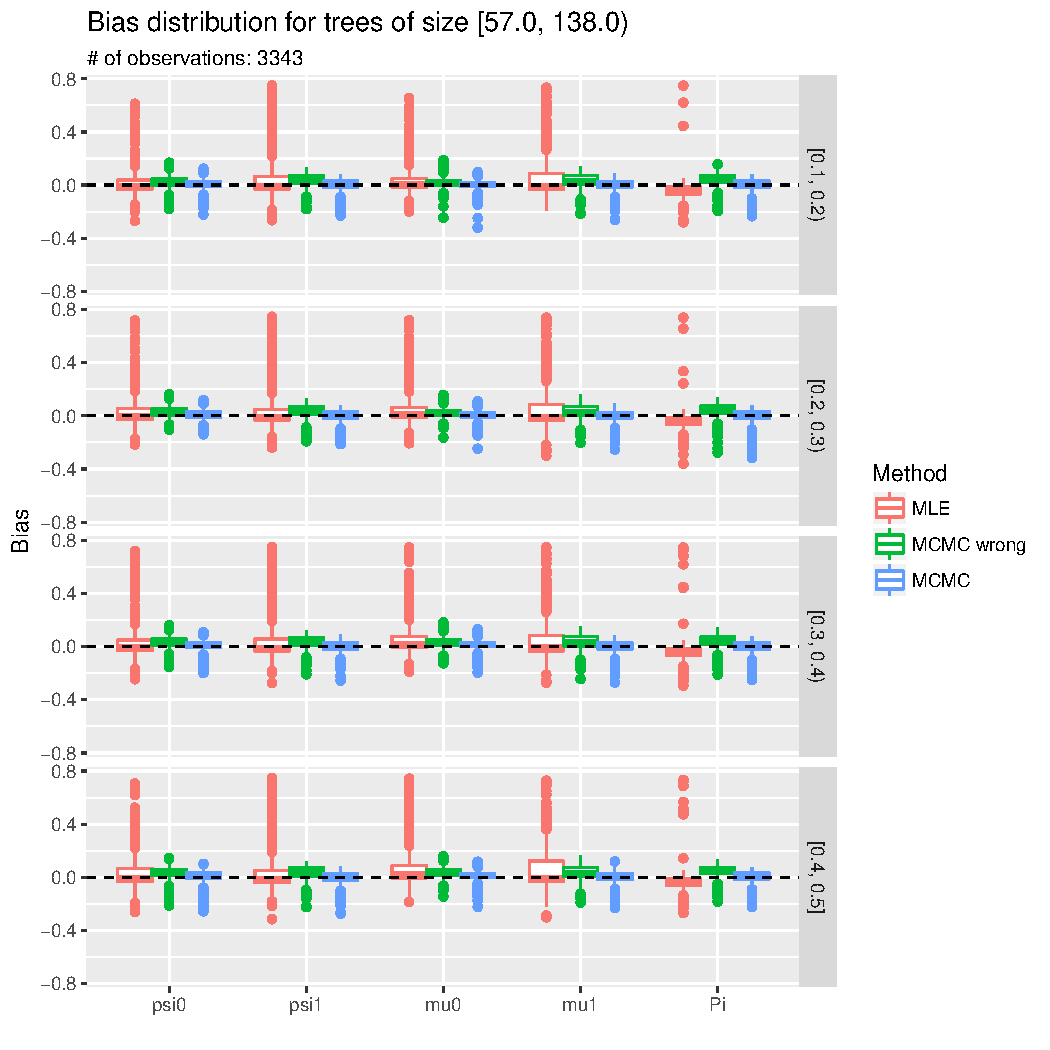
\includegraphics[width=.68\linewidth]{bias_trees_of_size_[57,138).pdf}
\end{figure}

\end{frame}

\begin{frame}[t]{A simulation study}

\framesubtitle{Convergence}

\begin{figure}
\centering
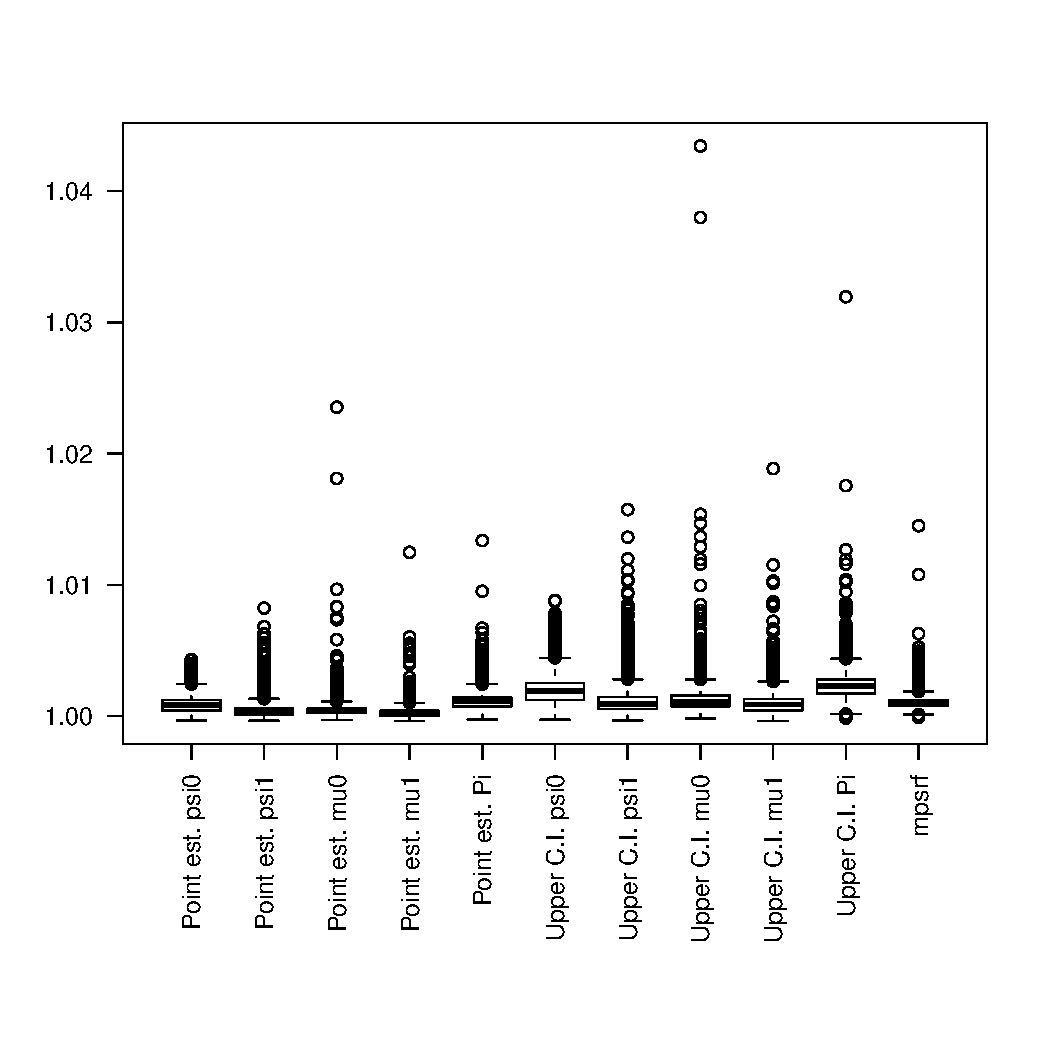
\includegraphics[width=.6\linewidth, trim={0 1.5cm 0 2cm},clip]{gelmans_right_prior.pdf}
\caption{Gelman diagnostic for convergence. The closer to 1, the better the convergence. Rule of thumb: A chain has a reasonable convergence if it has a Potential Scale Reduction Factor (PSRF) below 1.15.}
\end{figure}

\end{frame}

\begin{frame}[t]{A simulation study}

\framesubtitle{Prediction scores}

\begin{figure}
\centering
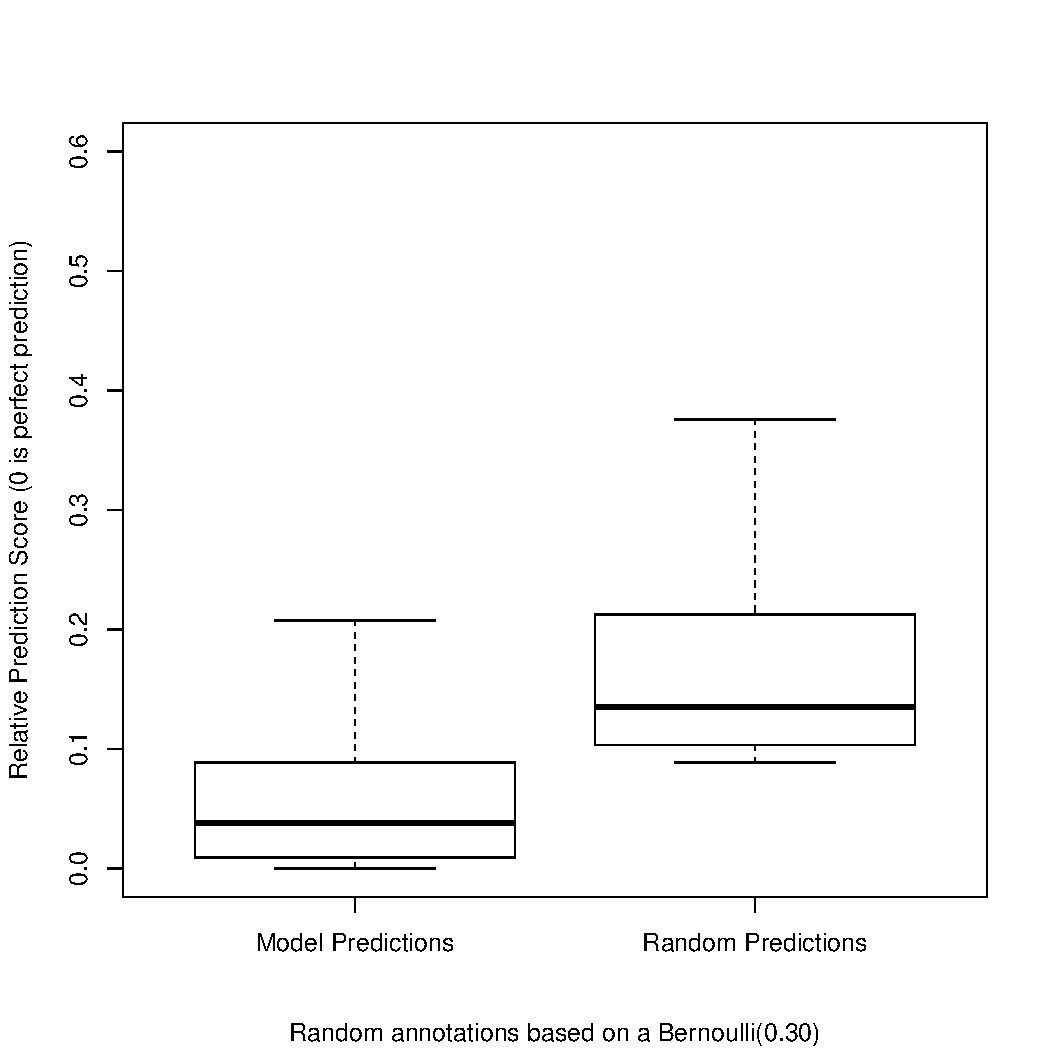
\includegraphics[width=.6\linewidth, trim = {0 1cm 0 2cm}, clip]{mcmc_right_prior_prediction.pdf}
\caption{Distribution of prediction scores. The random prediction scores were computed analytically with parameter $p=0.3$ (as resulting form the DGP).}
\end{figure}

\end{frame}

\section{Concluding Remarks}\label{concluding-remarks}

\begin{frame}{Concluding Remarks}

\begin{itemize}
\item
  A parsimonious model of gene functions: easy to apply on a large scale
  (we already ran some simulations using all 14,000 trees from the
  Panther DB).\pause
\item
  Already implemented, we are currently in the stage of writing the
  paper and setting up the simulation study.\pause
\item
  Unfortunately, since annotation data is so sparse, we lack of a
  significant number of useful datasets on which we can test our
  method.\pause
\item
  For the next steps, we are evaluating whether to include or how to
  include:\pause

  \begin{itemize}
  \item
    Type of node: speciation, duplication, horizontal transfer.
  \item
    Branch lengths
  \item
    Correlation structure between functions
  \item
    Using Taxon Constraints to improve predictions
  \end{itemize}
\end{itemize}

\end{frame}

\begin{frame}{}

\begin{center}
\Huge
\color{USCCardinal}{\textbf{Thank you!}}
\end{center}

\maketitle

\appendix

\end{frame}

\begin{frame}[t,label=formaldef]{Formal definitions}

\framesubtitle{\hyperlink{definitions}{\beamerbutton{go back}}}

\begin{enumerate}
\def\labelenumi{\arabic{enumi}.}
\item
  Phylogenetic tree: In our case, we talk about
  \textcolor{red}{partially ordered} phylogenetic tree, in particular,
  \(\phylo\equiv (N,E)\) is a tuple of nodes \(N\), and edges

  \[
  E\equiv \{(n, m) \in N\times N: n\mapsto m, \textcolor{red}{n < m}\}
  \]
\item
  Offspring of \(n\): \(O(n)\equiv\{m\in N: (n, m) \in E, n\in N\}\)
\item
  Parent node of \(m\): \(r(m) \equiv\{n \in N: (n, m) \in E, m\in N\}\)
\item
  Leaf nodes: \(\Leaf(\phylo)\equiv \{m \in N: O(m)=\{\emptyset\}\}\)
\item
  Annotations: Given \(P\) functions,
  \(\Ann \equiv \{\ann_n \in \{0,1\}^P: n\in \Leaf(\phylo)\}\)
\item
  Annotated Phylogenetic Tree \(\aphylo \equiv(\phylo, \Ann)\)
\item
  Observed Annotated Annotations
  \(\AnnObs = \{\annObs_l\}_{l\in \Leaf(\phylo)}\),
\item
  Experimentally Annotated Phylogenetic Tree
  \(\aphyloObs\equiv(\phylo, \AnnObs)\)
\end{enumerate}

\end{frame}

\begin{frame}[t,label=leafnodesprob]{Leaf node probabilities}

\framesubtitle{\hyperlink{peelingalgorithm<2>}{\beamerbutton{go back}}}

\begin{itemize}
\item
  The probability of the leaf nodes having annotations \(\ann_l\)
  conditional on the observed annotation is

  \begin{equation}
  \label{eq:leaf1}
  \Prcond{\Ann_{l} = \ann_{l}}{\AnnObs_{l} = \annObs_{l}} = \left\{
  \begin{array}{ll}
  \psi &\mbox{if }\annObs_{l} \neq \ann_{l} \\
  1 - \psi & \mbox{otherwise}
  \end{array}
  \right.
  \end{equation}

  Where \(\psi\) can be either \(\psi_0\) (mislabelling a zero), or
  \(\psi_1\) (mislabelling a one).
\end{itemize}

\end{frame}

\begin{frame}[t,label=internalnodeprob]{Internal node probabilities}

\framesubtitle{\hyperlink{peelingalgorithm<2>}{\beamerbutton{go back}}}

\begin{itemize}
\item
  In the case of the internal nodes, the probability of a given state is
  defined in terms of the gain/loss probabilities

  \[
  \Prcond{\Ann_{n} = \ann_{lp}}{\Ann_{r(n)} = \ann_{r(n)}} = \left\{
  \begin{array}{ll}
  \mu & \mbox{if }\ann_{n} \neq \ann_{r(n)} \\
  1 - \mu & \mbox{otherwise}
  \end{array}
  \right.
  \]

  Where \(\mu\) can be either \(\mu_0\) (gain), or \(\mu_1\) (loss).
\item
  Assuming independence accross offspring, we can write

  \begin{multline}
  \label{eq:interior1}
  \Prcond{\Ann_n = \ann_n}{\aphyloObs} = %
  \prod_{m \in O(n)} \sum_{\ann_m \in \{0,1\}} \Prcond{\Ann_m = \ann_m}{\aphyloObs} \\
  \Prcond{\Ann_{m} = \ann_{m}}{\Ann_{n} = \ann_{n}}
  \end{multline}

  Notice that if \(m\) is a leaf node, then
  \(\Prcond{\Ann_m = \ann_m}{\aphyloObs} = \Prcond{\AnnObs_m = \annObs_m}{\Ann_m = \ann_m}\).
\end{itemize}

\end{frame}

\begin{frame}[t,label=likelihood]{Likelihood of the tree}

\framesubtitle{\hyperlink{peelingalgorithm}{\beamerbutton{go back}}}

\begin{itemize}
\item
  Once the computation reaches the root node, \(n=0\), equations
  \eqref{eq:leaf1} and \eqref{eq:interior1}:

  \tiny

  \begin{align*}
  \Prcond{\Ann_l = \ann_l}{\aphyloObs} & = \Prcond{\Ann_{l} = \ann_{lp}}{\AnnObs_{l} = \annObs_{l}} \tag{\ref{eq:leaf1}}\\
  \Prcond{\Ann_n = \ann_n}{\aphyloObs}  & = 
  \prod_{m \in O(n)} \sum_{\ann_m \in \{0,1\}} \Prcond{\Ann_m = \ann_m}{\aphyloObs}  
  \Prcond{\Ann_{m} = \ann_{mp}}{\Ann_{n} = \ann_{n}} \tag{\ref{eq:interior1}}
  \end{align*}

  \normalsize

  Allow us writing the likelihood of the entire tree

  \begin{equation}
  \label{eq:l}
  \likelihood{\psi, \mu, \pi}{\aphyloObs} = \sum_{\ann_0\in\{0,1\}}\Prcond{\Ann_0=\ann_0}{\pi}\Prcond{\Ann_0=\ann_0}{\aphyloObs}
  \end{equation}

  Where
  \(\Prcond{\Ann_0=\ann_0}{\pi} = \pi^{\ann_{0}}\left(1 - \pi\right)^{1 - \ann_{0}}\)
\end{itemize}

\end{frame}

\end{document}
